%% \section{Results and Discussion}
%% \label{sec:results}

%% In this section we present the main findings of our research. We first present the results of each study (Section~\ref{sec:survey-resuts}, Sections~\ref{sec:msr-results}, and Section~\ref{sec:interview-results}). After that, in Section~\ref{sec:discussion} we consolidate our findings and present some implications of our study. 

\section{Results of the Survey}
\label{sec:survey-resuts} 

Our first study investigates the impact of atoms of confusion while developers try to understand JavaScript code.
We estimate this impact considering two perspectives: \emph{misunderstanding rate} (number of wrong answers)
and \emph{cognitive effort} (time necessary to provide a correct answer). 
We received full answers to our survey from 140 participants (a total of 70 replicas).
All participants had taken at least some university course or hold a bachelor
degree or equivalent, meaning the participants have had some level of formal education in programming. Twenty four participants hold either a master's degree (21 participants) or a doctorate degree (three participants). 
Considering the programming experience of our respondents, 19\% have more than ten years of programming experience, 37\% have between four and ten years of experience, 37\% have between one and four years of experience, and 7\% have less than one year of programming experience.  
Accordingly, we characterize the effect of atoms of confusion in JavaScript
code taking into account the perceptions of both novice and experienced developers. 

%Our audience comprises professional developers, and 93\% of the respondents have more than one year of experience with programming.
% (see Figure~\ref{fig:xp}). 
%Actually, 56\% of the participants have either between four and ten years of experience (37\%) or more than ten years of experience (19\%). Other 37\% of the respondents have between one and four years of experience.



%% Figure~\ref{fig:degree} and Figure~\ref{fig:xp} show the distributions of the subjects,
%% according to their education level and years of programming experience, respectively.

%% \begin{figure}[htb]
%%       \centering
%%       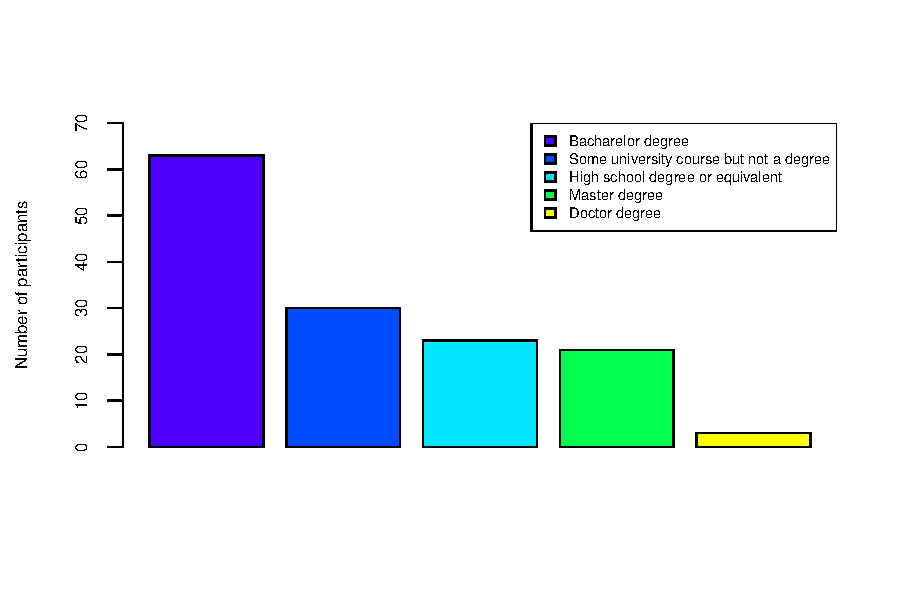
\includegraphics[width=\columnwidth]{images/dem-education-1.pdf}
%%       \caption{Participants' Education Level}\label{fig:degree}
%%   \end{figure}
  
%%   \begin{figure}[htb]
%%       \centering
%%       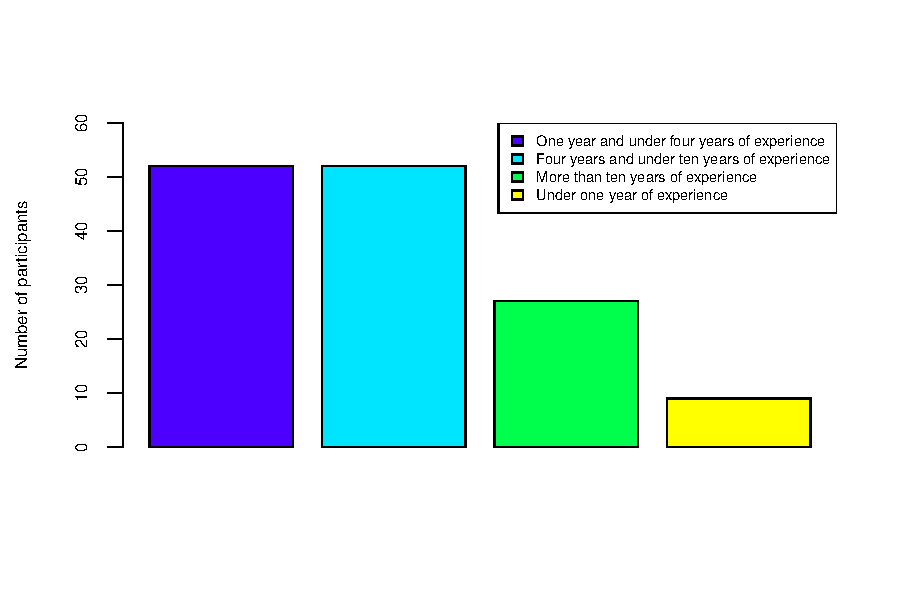
\includegraphics[width=\columnwidth]{images/dem-experience-1.pdf}
%%       \caption{Participants' Experience} \label{fig:xp}
%%   \end{figure}
%Figure~\ref{fig:xp} shows that more than a half of


\subsection{Misunderstanding Rate Analysis}

\subsubsection*{Exploratory Data Analysis}

As mentioned in Section~\ref{sec:meth:survey}, each participant in this study evaluated ten
code snippets, from which five were in their confusing versions, whilst the other five contained clean versions of the code snippets (i.e., without the confusing constructs and idioms). The participants should provide the expected outcomes of the code snippets. As discussed, we collected information about \emph{correctness} (whether the participant correctly predicted the program's output) and \emph{cognitive workload} (the time taken to answer the question). 
Table~\ref{tab:difference-correctness} and Figure~\ref{fig:boxplotcorrectness} summarize the results of the survey w.r.t. correctness.

Considering Table~\ref{tab:difference-correctness}, the clean versions of six code snippets present at least a 15\% improvement in answer correctness when compared with the confusing versions. In particular, the presence of the \emph{Comma Operator} atom presents the highest impact on misunderstanding. 
Frequently used constructs and idioms, such as \emph{Post Increment} and \emph{Omitted Curly Braces} (see Section~\ref{sec:msr-results}), also result in many mistakes. %introduce high degrees of confusion.
The boxplot of Figure~\ref{fig:boxplotcorrectness} shows a non-negligible decrease in the average number of incorrect answers when observing the clean versions of the code snippets. Also, the sample of responses with no atoms had almost no dispersion, which supports the
argument that the non-confusing versions of the code snippets are easier to evaluate correctly. 


% \begin{table}[htbp]
% \caption{Difference in answer correctness between confusing and non-confusing pairs}
% \begin{center}
% \begin{small}
% \begin{tabularx}
% {{\linewidth}}{l p{1.5cm} p{1.1cm} p{1.1cm} p{1.2cm} }
% \textbf{Atom} & \textbf{\%Correct} & \textbf{\%Correct} \\
% &  \multicolumn{1}{l}{With AOC} \multicolumn{2}{l}{Without AOC}  & \Delta (\%)    \\
%  \hline
% Comma Operator & 40 & 93 & +132\%                 \\     
% Automatic Semicolon  Insertion & 46 & 97 & +110\% \\
% Post Increment & 69 & 91 & +31\%         \\
% Omitted Curly Braces & 67 & 83 & +23\%   \\ 
% Assignment as Value & 80 & 97 & +21\%    \\
% Implicit Predicate & 83 & 97 & +16\%     \\
% Logic as Control Flow & 59 & 68 & +15\%  \\
% Ternary Operator & 86 & 94 & +9\%        \\
% Pre-Increment & 71 & 76 & +7\%           \\
% Arithmetic as Logic & 91 & 90 & -1\%    \\
% \end{tabularx}
% \end{small}
% \end{center}
% \label{results_correctness}
% \end{table}

\begin{table}[htbp]
\caption{Total number of correct answers}
\label{tab:difference-correctness}
\centering{
\begin{scriptsize}
\begin{tabular}{lccc} \toprule
  Atom & Confusing Code & Clean Code & $\Delta$(\%)  \\ \midrule
  Comma Operator                &  28 &  65 & +132   \\ 
  Automatic Semicolon Insertion &  32 &  68 & +112   \\ 
  Post-Increment                &  48 &  64 & +33    \\ 
  Omitted Curly Braces          &  47 &  58 &  +23   \\
  Assignment as Value           &  56 &  68 &  +21   \\ 
  Implicit Predicate            &  58 &  68 &  +17   \\ 
  Logic as Control Flow         &  41 &  48 &  +17   \\ 
  Ternary Operator              &  60 &  66 &  +10   \\ 
  Pre-Increment                 &  50 &  53 &  +6    \\ 
  Arithmetic as Logic           &  64 &  63 &  -2    \\ \bottomrule
  
\end{tabular}
\end{scriptsize}
}
\end{table}

 %% Comma Operator          & 40 & 93  & +132 \\
 %% Post Increment          & 69 & 91  & + 31  \\
 %% Omitted Curly Braces    & 67 & 83  & +23 \\
 %% Assignment as Value     & 80 & 97  & +21 \\
 %% Implicit Predicate      & 83 & 97  & +16 \\
 %% Logic as Control Flow   & 59 & 68  & +15 \\
 %% Ternary Operator        & 86 & 94  & +9  \\
 %% Pre-Increment           & 71 & 76  & +7  \\
 %% Arithmetic as Logic     & 91 & 90  & +1  \\ \bottomrule


\begin{figure}[htb!]
\noindent
 \centering
 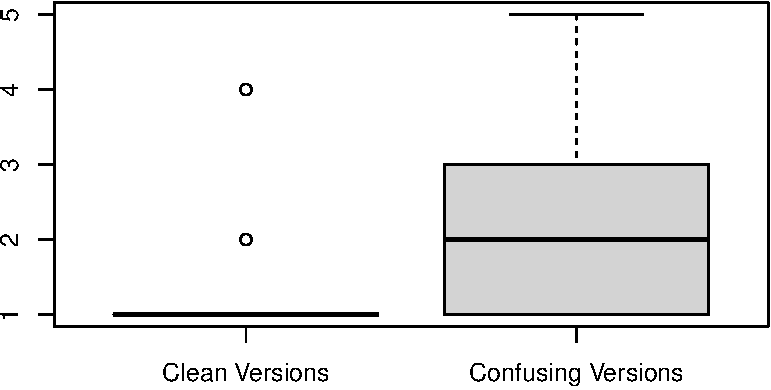
\includegraphics[width=\columnwidth]{images/wrong-answers-plot-1.pdf}
 \caption{Number of wrong answers of each subject.}
 \label{fig:boxplotcorrectness}
 \end{figure}

% \rb{verificar a consistencia nas questoes de pesquisa mais especificas}

\subsubsection*{Hypothesis Testing and Effect Size}

We first use the \emph{Pearson's Chi-squared test}
to investigate if there is a statistically significant difference in the frequency of correct and incorrect answers---due to the versions of the code snippets (confusing and clean code). The p-values for these tests are reported in the ``Chi-square test'' column of Table~\ref{tab:hypothesis-testing}. The results indicate that for five atom candidates (Comma Operator, Automatic Semicolon Insertion, Post-Increment, Assignment as Value, Implicit Predicate) the confusing versions of the code snippets have a negative impact on code understanding (p-value $< 0.05$). This result holds even after applying the Benjamini-Hochberg correction with a false discovery rate of 5\%. 

We measure the effect size of the clean version of the code snippets into the answers' correctness using the \emph{Odds Ratio} (OR). The results are reported in the ``Odds Ratio'' column of Table~\ref{tab:hypothesis-testing}. In the table, we also report the confidence interval (CI) for the OR in the ``CI'' column. Although many of the intervals are wide, for six of the atom candidates the lower bound of the confidence interval is greater than or equal to 1. This indicates that, at a 95\% confidence level, a developer is likely to commit less mistakes when using the clean versions.
%We found a negligible effect size for the atom candidates Arithmetic as Logic, Logic as Control Flow, and Pre-Increment. Nonetheless, for the remaining candidates, the effect size is significant. 
For instance, when comparing clean and confusing code snippets pertaining to the Comma Operator atom candidate, we observed an \emph{Odds Ratio} of \num{19.02}. This means that the odds of a correct answer are \num{19.02} times higher when interpreting the clean version---in comparison with the corresponding confusing version of the code snippet. Furthermore, with a 95\% confidence level, the odds  ratio is between 6.6 and 68.22, i.e., although the error margin is wide, it is strongly in favor of the clean version. If there is a significant likelihood of a developer committing a mistake when analyzing a clean version, the lower bound of the CI should be a number between 0 and 1 (since the OR is a ratio). This is the case for the four atom candidates in the lower part of the table. In particular, in the last row (Arithmetic as Logic), the OR between 0 and 1 indicates that a study subject was actually more likely to misunderstand the clean version. 

Finally, we also use the \emph{Binomial Generalized Logistic Regression} analysis to investigate if either participant \emph{education} or participant \emph{experience} impact correctness. Although the results suggest that experience impacts correctness, the education level does not. As such, we replicate the \emph{Pearson's Chi-squared test} for each experience group and found that the statistical difference is less significant for those developers with more than ten years of experience. 

\begin{mh}
  The results of our exploratory data analysis and
  hypothesis testing suggest that the atom
  candidates Comma Operator, Automatic Semicolon Insertion, Post Increment, Omitted Curly Braces, 
  Assignment as Value, and
  Implicit Predicate %, and Ternary Operator
  introduce some degree of misunderstanding
  in JavaScript code. %Based on the results of this study, 
  Therefore, they can be deemed atoms of confusion for JavaScript.
\end{mh}

%% Regarding the first question we 
%% address in the survey (\emph{Do code snippets that contain atoms of confusion produce a higher error rate than snippets where the atom is removed?}), we found evidence that the atoms of confusion lead programmers to misunderstand JavaScript code. We also realized that just one atom whose correction has a non-significant improvement in the percentage of correct answers---we found an improvement of at least 15\% in the correct answers when removing the confusing code for seven atoms (out of ten atoms we consider in the survey). 

\subsection{Cognitive Workload Analysis}

\subsubsection*{Exploratory Data Analysis}
Table \ref{tab:difference-time-taken} shows the average time necessary for the participants to give a correct answer about the expected outcomes of a code snippet, considering both confusing and clean versions. Seven atom candidates require an increasing cognitive workload. For these seven atom candidates, developers take at least 5.90\% less time on average to find a correct answer when considering the clean version of a code snippet. In the extreme case (atom candidate Comma Operator), the participants take 76.23\% less
time on average to find the correct answer for the clean version of the code snippets. 
Not all atom candidates, though, require less time for the participants to predict the answer. In fact, for the Arithmetic as Logic and the Pre-Increment atoms, the time to give a correct answer increased  
29.06\% and 38.19\% for the clean versions.

\begin{table}[htbp]
\caption{Time in seconds to submit a correct answer}
\label{tab:difference-time-taken}
\centering{
\begin{scriptsize}
\begin{tabular}{lccc} \toprule
Atom & Confusing Code & Clean Code & $\Delta$(\%) \\ \midrule
Comma Operator & 87.67 & 20.84 & -76.23 \\ 
Automatic Semicolon Insertion & 46.08 & 22.04 & -52.17 \\ 
Post-Increment & 28.70 & 25.67 & -10.56 \\ 
Omitted Curly Braces & 48.85 & 30.00 & -38.58 \\ 
Assignment as Value & 52.47 & 48.95 & -6.71 \\ 
Implicit Predicate & 36.24 & 24.01 & -33.75 \\ 
Logic as Control Flow & 108.94 & 51.07 & -53.12 \\ 
Ternary Operator & 41.80 & 39.34 & -5.90 \\ 
Pre-Increment & 30.71 & 42.45 & 38.19 \\  
Arithmetic as Logic & 28.82 & 37.20 & 29.06 \\ \bottomrule
\end{tabular}
\end{scriptsize}
}
\end{table}

 % latex table generated in R 4.0.4 by xtable 1.8-4 package
 % Thu Apr 22 07:58:21 2021
 \begin{table*}[ht]
\caption{Hypotheses Testing (misunderstanding and cognitive workload)}
\label{tab:hypothesis-testing}

 \centering
 \begin{tabular}{lccc|cc}
   \toprule
Atom  & Chi-square test & Odds Ratio          & CI & Mann-Whitey U test & Cliff's Delta \\ 
     &         & (misunderstanding)  &                    & (workload)             & \\ \midrule
Comma Operator & 1.1727e-10 & 19.02 & (6.60, 68.22) & 5.8249e-08 & -0.53 \\ 
Automatic Semicolon Insertion & 5.8352e-11 & 39.33 & (9.21, 356.62) & 0.09802 & -0.16 \\ 
Post-Increment & 0.0015279 & 4.83 & (1.73, 15.74) & 0.12006 & 0.15 \\ 
Omitted Curly Braces & 0.050962 & 2.35 & (1.00, 5.77) & 0.92529 & -0.01 \\ 
Assignment as Value & 0.0034775 & 8.39 & (1.81, 79.12) & 0.82681 & 0.02 \\ 
Implicit Predicate & 0.01123 & 6.95 & (1.46, 66.56) & 0.0029039 & -0.29 \\ 
Logic as Control Flow & 0.292 & 1.54 & (0.73, 3.28) & 7.5862e-05 & -0.39 \\ 
Ternary Operator & 0.15896 & 2.73 & (0.74, 12.57) & 0.24073 & -0.12 \\ 
Pre-Increment & 0.70147 & 1.25 & (0.55, 2.85) & 0.0062981 & 0.27 \\ 
Arithmetic as Logic & 1 & 0.84 & (0.22, 3.12) & 0.01723 & 0.23 \\ 
    \bottomrule
 \end{tabular}
 \end{table*}


\subsubsection*{Hypothesis Testing}
We use the non-parametric \emph{Mann-Whitney U test}, also known as Wilcoxon rank-sum test, to
investigate the null hypothesis that developers 
spend the same amount of time to correctly
predict the outcome of a code snippet, regardless
of evaluating the confusing or  clean version
of the code. The results of Table~\ref{tab:difference-time-taken}
suggest that we should refute the null hypotheses for
six atom candidates (Comma Operator, Automatic Semicolon Insertion,
Implicit Predicate, Logic
as Control Flow, Pre-Increment, and Arithmetic
as Logic). For the first four, the analysis suggests that the participants
need more time to predict the outcome of
the code snippet in the confusing code version. Interestingly, for the atom candidates Arithmetic as Logic and Pre-Increment, the participants take less time
to predict the outcome of the code snippets in
the confusing version.
We also computed the effect size using the Cliff's Delta method. We found a large effect for the Comma Operator atom candidate; and a moderate effect for the atom candidates
Logic as Control Flow, Implicit Predicate, Arithmetic
as Logic, and Pre-Increment. 


\begin{mh}
  The results suggest that developers spend
  significantly more time to predict the
  correct answer in the presence of the
  atom candidates Comma Operator, Automatic Semicolon Insertion, Logic as
  Control Flow, and Implicit Predicate. Conversely,
  the code snippets with the
  atom candidates Arithmetic as Logic and
  Pre-Increment demand less time to
  predict the correct answers. 
\end{mh}


%%  Comma Operator        & 60 & 21  & -65  \\
%% Logic as Control Flow & 85 & 49  & -42  \\
%% Implicit Predicate    & 33 & 24  & -27  \\
%% Omitted Curly Braces  & 43 & 31  & -27  \\
%% Assignment as Value   & 53 & 49  & -7   \\
%% Ternary Operator      & 42 & 42  & 0    \\
%% Post Increment        & 27 & 27  & 0    \\
%% Arithmetic as Logic   & 29 & 36  & +24  \\
%% Pre-Increment         & 34 & 49  & +44  \\


\
% \rb{acho que podemos melhorar a apresenta\c c\~{a}o dessas tabelas, talvez usando booktabs.}


\section{Results of the Interview Study}
\label{sec:interview-results}

%% \rb{acho que essa separa\c c\~{a}o em dois rounds est\'{a}
%%   gerando uma complexidade desnecess\'{a}ria. vou tentar
%%   remover isso}.

In this section, we present the results of the 
interviews with the 15 practitioners who agreed to participate
in the study. 
% A total of 15 practitioners took part of the interviews.
We collected information regarding programming
experience, familiarity with JavaScript, and their opinion
about the \na atom candidates we explored in our research.
We first present them pairs of clean and confusing code snippets 
and then ask them to discuss their preferences towards one version.
% ask the participants to discuss their preferences (i.e., code with or without atom).


%% In the second round of interviews, ten of the fifteen developers
%% who participated in the first round were shown another 8 atom candidates to atom of confusion whose frequency we observed during the repository mining phase. The same procedure of showing code that behaves exactly the same and surveying for how easy to understand each snippet was applied in this phase. 

\subsubsection*{The Participants' perceptions of the atom candidates}
Supporting the results of the survey, Table~\ref{tab:interview-results1}
 shows that for eight out of the
10 scenarios surveyed, the majority of the respondents prefer the version of the
code without the atom of confusion.
In no case the \emph{neutral}
ratio was higher than the option for the version without atoms of confusion.
%% An example entry is contained in Appendix~\ref{}. 
%% For a full listing of the code snippets, visit the paper repository. 
Only for the Ternary Operator atom candidate the participants
prefer the version of the code with the atom of confusion,
instead of the version without the atom of confusion.
We show the code snippets for the Ternary Operator in Figure~\ref{code:ternary}.
Even for this atom candidate, some participants who preferred 
the \emph{left-hand-side} version (with the atom of confusion) 
still believed that the \emph{right-hand-side} version (without the atom of
confusion) was more readable.  
The following quotes were extracted from the transcripts with
% three interviewees:
two interviewees:

\begin{figure*}

\noindent\begin{minipage}{.45\textwidth}
\begin{lstlisting}[language=JavaScript, caption=\emph{Left-hand side} (using the \emph{Ternary Operator} atom).]
let config = {size: 3, isActive: false};
const_config = config.isActive === true 
             ? config 
             : {size: 10};
console.log(_config.size);
\end{lstlisting}
\end{minipage}\hfill
\begin{minipage}{.45\textwidth}
\begin{lstlisting}[language=JavaScript, caption=\emph{Right-hand side} (without the atom).]
let config = {size: 3, isActive: false}
let _config;
if(config.isActive === true) {
  _config = config;
}
else{
   _config = {size: 10};
}
console.log(_config.size);
\end{lstlisting}
\end{minipage}
\caption{Example of pair of code snippets used in the interview. This case explores the use of the \emph{Ternary Operator atom of confusion}}
\label{code:ternary}
\end{figure*}

\begin{mq}
\emph{``I prefer to write [code using the \lhs version], but I think [the \rhs version] is easier to read, especially for newer programmers''}.
\end{mq}

\begin{mq}
\emph{``When I am programming, I write code with the ternary operator, [...], but, to be honest, I still think that the 
[the code using the \lhs version] 
is easier to understand''}.
\end{mq}

%% \begin{mq}
%% \emph{``I think [the \lhs version] is easier to understand, but [the \rhs version] is what I would write"}
%% \end{mq}

%% The atom candidate Ternary Operator also opens up
%% the possibility for a derivative construct that JavaScript
%% allows which can be rather confusing, and that is the nested
%% ternaries construct, in which the right-hand side of the a
%% ternary operator can be another ternary construct.
%% While nested ternaries remove the number of lines that
%% would be necessary to construct using nested if-then-else statements,
%% they can become quite taxing to understand.
%% Nested ternaries are a choice of atoms to be analyzed in future work.

The Pre-Increment atom candidate also caused such
divide in one of the interviewees, as they
regarded the \emph{\rhs version} (without atom of confusion)
as simpler to understand, but would still opt to write
code with the atom. In contrast, %to such opinion,
one of the participants found the 
version with the atom of confusion more elegant,
but recognized it was less readable,
and was willing to sacrifice elegance for readability.

%% \rb{pela discuss\~{a}o anterior, parece-me que alguns
%%   desenvolvedores reconhecem que esses candidatos
%%   a \'{a}tomos introduzem certa dificuldade de compreens\~{a}o;
%%   mas mesmo assim optam por usar a constru\c c\~{a}o correspondente.
%%   Acho que cabe um box aqui com essa discuss\~{a}o sobre isso.}

When analyzing the Logic as Control Flow atom candidate, one of
the interviewees gave an example of his own experience
that might motivate one to avoid writing code using this construct:

\begin{mq}
  \emph{``This one is interesting, because I have written
  code that looks like the [\lhs version (with the atom of confusion)],
  and my colleagues complained that it was difficult to understand.
  Nowadays I prefer to write code using the [\rhs version]"}.
\end{mq}

Two of the atom candidates had unanimous preference for the
versions that did not contain the atoms: Comma Operator and
Omitted Curly Braces. Regarding the first one, we could
often notice during the interviews that
the \emph{\lhs} (with the atom of confusion) 
caused significant
confusion among the participants. One remark about
the \emph{Comma Operator} atom of confusion is listed below:

%% \begin{mq}
%% \emph{``I just learned that [the \lhs version of this code] is possible. I did not even know it worked''}
%% \end{mq}

\begin{mq}
\emph{``The code in 
[the \lhs version]
is unlikely to be understood unless the programmer knows \clang or \cpplang''}.
\end{mq}

As for the atom candidate Omitted Curly Braces, one of the interviewees mentioned that, although they understand why one would opt not to use braces for simple if-then-else statements, he still advised against it, on grounds that:

\begin{mq}
\emph{``[I prefer the \rhs version of the code \ldots]
If I want to see well-written, easily understandable code, then I also have to do my job. Therefore I believe that, since I do not know who is on the other end maintaining this code, and it could be any person with any level of expertise, then I try to write readable, easy-to-understand code''}.
\end{mq}

%This is an interesting perspective, because such a perhaps simple decision,  might hinder novice developers in the task of maintaining code; and one cannot make any assumption about the programmers' experience of who is going to maintain a code in a long run.

This is an interesting perspective because such a perhaps simple decision might hinder novice developers in maintaining code; one cannot assume the programmers' experience of who will maintain a code in the long run.

\begin{table}[!htb]
    \centering
    \caption{Summary of participants' preferences for code snippets \emph{with} (LHS) and
      \emph{without} atoms of confusion (RHS).
      Participants were also allowed to choose NEUTRAL when they thought both sides were equally readable.}
    \label{tab:interview-results1}
    \begin{tabular}{lrrr}\toprule
      & \multicolumn{3}{c}{\textsc{Preference (\%)}} \\
      \cmidrule(lr){2-4}
         Atom           & \multicolumn{1}{c}{\textsc{LHS}}
                                      &  \multicolumn{1}{c}{\textsc{RHS}}
                                               & \multicolumn{1}{c}{NEUTRAL} \\ \midrule
         Comma Operator                  & 0  & 100    & 0     \\
         Automatic Semicolon Insertion  & 0  & 80     & 0     \\
         Post-Increment                  & 20 & 73.33  & 6.67  \\
         Omitted Curly Braces            & 0  & 100    & 0     \\
         Assignment as Value             & 20 & 60     & 20    \\
         Implicit Predicate              & 20 & 73.33  & 6.67  \\
         Logic as Control Flow           & 20 & 60     & 20    \\
         Ternary Operator                & 60 & 26.67  & 13.3  \\
         Pre-Increment                   & 40 & 46.67  & 13.33 \\ 
         Arithmetic as Logic             & 0  & 93.33  & 6.67  \\ \midrule
         \textsc{overall}                & 18 & 71.33  & 8.64  \\
         \bottomrule
    \end{tabular}
\end{table}


\subsubsection*{Confusion in JavaScript Code} 

% The final remarks that were drawn from the interviews are related to potentially confusing constructs that were suggested by the participants, as well as their perspective on JavaScript as a language, from which we can also uncover some other forms in which the language itself might contribute to writing confusing code.

The final remarks drawn from the interviews are related to potentially confusing constructs suggested by the participants and their perspectives on JavaScript as a language.
From the latter, we can also uncover some other forms in which the language itself might contribute to writing confusing code.

One of the participants mentioned that the use of JavaScript's prototype-based inheritance can make it difficult to understand code, particularly when involving  deep prototype chains. This is a core feature of the language, and most high-level tools and frameworks abstract it away. Although this was only mentioned by one practitioner, this is an important remark, as true understanding of JavaScript software necessarily involves understanding the concept of prototypes.

% When asked about particular JavaScript constructs or patterns that can make code difficult to understand, three participants cited the callback pattern, which can lead to several levels of nested function calls, as extremely difficult to assimilate.
When asked about particular JavaScript constructs or patterns that can make code difficult to understand, three participants cited the callback pattern---potentially leading to several levels of nested function calls---as extremely difficult to assimilate. 
One of the respondents stated:

\begin{mq}
\emph{``Nested callbacks are very confusing. Even writing them can be confusing, let alone understanding them.''}
\end{mq}

Two other developers implicitly touched upon the callback pattern, mentioning that it can be difficult to understand \emph{asynchronous} programming in JavaScript. Since what is really happening at a lower level is that the JavaScript engine creates a callback stack that is separate from the main execution stack, and that callback functions are only executed when the main execution stack is empty, the concepts of asynchronous events and callbacks are inseparable in the language, and any abstractions for callback functions, such as promises and async/await syntax only hide the pattern. We also found other idioms that are JavaScript atom candidates, including
\emph{property access} via array subscription (\lstinline[language=javascript]{V1['P1']} instead of \lstinline[language=javascript]{V1.P1}) and \emph{arrow functions} (see listings~\ref{arr1} and~\ref{arr2}). 

\begin{figure}
\begin{small}
\begin{lstlisting}[language=JavaScript,caption=Example of arrow function.,label=arr1]
let inc = (x) => x + 1;
\end{lstlisting}
\begin{lstlisting}[language=JavaScript,caption=Alternative version without arrow function.,label=arr2]
let inc = function(x) {
  return x + 1
}
\end{lstlisting}
\end{small}
\end{figure}


% citar uninitialized objects' types. floating point precision issues, 'this', type coercion

% \subsection{Common Misunderstandings About the Language}

% TODO: I don't see that our results support these claims.
% Let us comment for now.

%% Six practitioners regarded the JavaScript language as easy to learn, while four
%% participants mentioned that the abundance of frameworks,
%% coupled with the abstractions they provide, make it so that one
%% can develop quickly in the language. However, as mentioned by one
%% of the interviewees, ``\emph{Developers who have started
%% programming in JavaScript might miss out on important lower-level
%% aspects, such as garbage collection, memory management,
%% and process management.}''. 

%% Moreover, such abstractions might lead a developer to start to program
%% using the language without actually understanding some of its basic aspects.
%% For instance, four participants argued that the language is not typed, two  believed the language runs exclusively on browsers, and two other developers stated that the language is natively asynchronous, all of which are incorrect statements.
%% For the multi-purpose language that is one of the most, if not the most used one by practitioners,
%% a lack of understanding of the languages core
%% features may be a problem worth investigating in future studies.



%% \begin{table}[!htb]
%%     \centering
%%     \caption{Interviews Round 2 - Summary of participants' preferences for code snippets \textsc{with} and \textsc{without} atoms of confusion (\textsc{aoc}). Participants were also allowed to choose \textsc{neutral} when they thought both sides were equally readable.}
%%     \label{tab:interview-results2}
%%     \begin{tabular}{lrrr}\toprule
%%       & \multicolumn{3}{c}{\textsc{Preference (\%)}} \\
%%       \cmidrule(lr){2-4}
%%          \textsc{atom}           & \multicolumn{1}{c}{\textsc{with aoc}}
%%                                       &  \multicolumn{1}{c}{\textsc{without aoc}}
%%                                                & \multicolumn{1}{c}{\textsc{neutral}} \\ \midrule
%%          Property access         & 10  & 60  & 30  \\
%%          Object spread           & 50 & 50     & 0    \\
%%          Array spread            & 60  & 40    & 0     \\
%%          Arrow function          & 40 & 40     & 20  \\
%%          Array destructuring     & 40 & 40  & 20  \\
%%          Object destructuring    & 40 & 40     & 20    \\
%%          Type conversion         & 30  & 60    & 10     \\
%%          Change Literal encoding & 40 & 50  & 10  \\ \midrule
%%          \textsc{overall}        & 42.8 & 47.6  & 9.6  \\
%%          \bottomrule
%%     \end{tabular}
%% \end{table}

\section{Results of the MSR Effort}
\label{sec:msr-results} 

We mined \minedprojects open source JavaScript repositories to understand how
often atoms of confusion arise in real software. 
Similarly to previous studies~\cite{DBLP:conf/msr/GopsteinZFC18,DBLP:journals/ese/MedeirosLAAKRG19}, which investigate
the prevalence of atoms of confusion in open source \clang and \cpplang projects, we found that atoms of confusion
frequently arise in JavaScript open source systems. For instance, the six most frequently found atoms
occur in at least 80\% of the projects. Considering the extremes, atoms Ternary Operator and Implicit Predicate were found in all repositories we mined,
while atom Comma Operator occurred in only 15\% of them (as seen in Table~\ref{tab:occurrences-summary}).

% Figure~\ref{fig:rate} summarizes this finding, showing that the occurrence of atoms of confusion in JavaScript systems range from 11.34\% (Comma Operator) to 89.69\% (Ternary Operator).


%Figure~\ref{fig:atoms-occurrence} shows that the occurrence of in JavaScript systems range from 

% latex table generated in R 4.0.3 by xtable 1.8-4 package
% Fri Nov 13 11:28:56 2020
%%\begin{table}[!htb]
%%\centering
%% \caption{Summary of atoms occurrences on our dataset}
%% 
%%\setlength\tabcolsep{2pt} % default value: 6pt
%%\label{tab:occurrences-summary}
%%\begin{tabular}{lrcc}
%%
%%  \hline
%%Atom & Projects & Occurrences/KLOC & Category \\ 
%% \hline
%%Ternary Operator & 100\% & 10.16 &  highly used \\ 
%%Omitted Curly Braces & 91.67\% & 6.61 &  highly used \\ 
%%Post Increment & 90.28\% & 5.62 &  highly used \\ 
%%Pre-Increment & 83.33\% & 1.04 & commonly used \\ 
%%Assignment as Value & 81.94\% & 1.02 & commonly used \\ 
%%Logic as Control Flow & 56.94\% & 0.95 & commonly used \\ 
%%Arithmetic as Logic & 23.61\% & 0.02 & little used \\ 
%%Comma Operator & 15.28\% & 0.03 & little used \\ 
%%   \hline
%%\end{tabular}
%%\end{table}

% latex table generated in R 4.0.3 by xtable 1.8-4 package
% Tue Apr 13 09:34:35 2021
\begin{table}[ht]
\centering
\caption{Summary of atoms occurrences on our dataset}
\setlength\tabcolsep{2pt} % default value: 6pt
\label{tab:occurrences-summary}
\begin{tabular}{lrcc}
  \toprule
Atom & Projects & Occurr./KLOC & Frequency \\ 
  \midrule
Implicit Predicate & 100\% & 19.89 &  highly used \\ 
  Ternary Operator & 100\% & 10.16 &  highly used \\ 
  Omitted Curly Braces & 91.67\% & 6.61 &  highly used \\ 
  Post Increment & 90.28\% & 5.62 &  highly used \\ 
  Pre Increment & 83.33\% & 1.04 & commonly used \\ 
  Assignment as Value & 81.94\% & 1.02 & commonly used \\ 
  Logic as Control Flow & 56.94\% & 0.95 & commonly used \\ 
  Automatic Semicolon Insertion & 33.33\% & 0.13 & commonly used \\ 
  Arithmetic as Logic & 23.61\% & 0.02 & little used \\ 
  Comma Operator & 15.28\% & 0.03 & little used \\ 
   \bottomrule
\end{tabular}
\end{table}


Considering all JavaScript projects in our dataset, we found 
a total of \num{364873} atoms of confusion, though four atoms are responsible
for 92.97\% of this total: Implicit Predicate, Ternary Operator, Omitted Curly Braces, and the Post Increment. The remaining atoms
account for \num{25621} (7.03\%) of the total number of occurrences.
Moreover, the Comma Operator and Arithmetic as Logic atoms are the ones that arise less
frequently (0.001\% in total with 232 and 165 occurrences, respectively). 

Regarding frequency, we proceeded with a classification of \emph{atom occurrence}
according to the thresholds of a previous
study~\cite{DBLP:journals/ese/MedeirosLAAKRG19}. 
In particular, atoms with less than \num{1000} occurrences are classified as \textit{little used}, while atoms with more than \num{10000} occurrences are classified as \textit{highly used}; \textit{commonly used} atoms occur in between.
We found four
atoms as highly used (Implicit Predicate, Ternary Operator, Omitted Curly Braces, and Post Increment),
four as commonly used (Pre-Increment, Assignment as Value,
Logic as Control Flow, and Automatic Semicolon Insertion),
and two atoms as little used (Arithmetic as Logic and Comma Operator).
We also calculated the frequency of each atom per KLOC and found the atoms
Implicit Predicate (19.89 occurrences per KLOC) and Ternary Operator (10.16
occurrences per KLOC) as the most occurring
in practice.
%In our dataset of JavaScript projects, 
%We found the Ternary Operator atom occurring more frequently than the Omitted Curly Braces, differently from what has been reported in a previous work~\cite{DBLP:conf/msr/GopsteinZFC18}. %

The results of our survey and interviews suggest that the
Ternary Operator does not contribute significantly as a source of
misunderstanding (increasing the number of wrong answers in 9\% of the cases,
according to our survey). 
Nonetheless, the Post-Increment Expression
and Omitted Curly Braces atoms are listed in the top four sources of misunderstanding 
(see Table~\ref{tab:difference-correctness}), and also frequently appear
in open source systems. As such, fixing the
the Post-Increment and Omitted Curly Braces might improve a considerable
amount of unclear code caused by atoms of confusion in
JavaScript projects. 
